\subsection{Very simple linear test case}

\begin{frame}{What is the purpose of enrichment?}

\vspace{-5pt}
\only<1-2>{\textbf{Poisson problem} (with Dirichlet BC) \textbf{:} \; Find $u : \Omega \rightarrow \mathbb{R}$ such that
\vspace{-5pt}
\begin{equation*}
    \left\{
    \begin{aligned}
        -\Delta u & = f, \; &  & \text{in } \; \Omega, \\
        u         & =0, \;  &  & \text{on } \; \partial\Omega.
    \end{aligned}
    \right.
    % \label{eq:Lap2D}\tag{$\mathcal{P}$}
\end{equation*}}

% \only<2>{\textbf{\textcolor{darkred}{Modified} Poisson problem :} \; Find $\textcolor{darkred}{C_{h,u}^+} : \Omega \rightarrow \mathbb{R}$ such that
% \vspace{-5pt}
% \begin{equation*}
%     \left\{
%     \begin{aligned}
%         -\Delta \textcolor{darkred}{C_{h,u}^+} & = f + \textcolor{darkred}{\Delta u_\theta}, \; &  & \text{in } \; \Omega, \\
%         \textcolor{darkred}{C_{h,u}^+} & =0, \;  &  & \text{on } \; \partial\Omega,
%     \end{aligned}
%     \right.
%     % \label{eq:Lap2D}\tag{$\mathcal{P}$}
% \end{equation*}
% with $u_{\theta}$ a PINN prediction.}

\only<1-2>{\textbf{Variational Problem :} We consider $V_h^0$ a $\mathbb{P}_k$ continuous Lagrange FE space ($k\geq 1$).
\begin{equation}
    \label{eq:weakform}
    \text{Find } u_h\in V_h^0 \;\text{such that}, \forall v_h\in V_h^0, a(u_h,v_h)=l(v_h),
    \tag{$\mathcal{P}_h$}
\end{equation}
\vspace{1pt}
with $h$ the characteristic mesh size, $a$ and $l$ the associated bilinear and linear forms.}

\only<2-3>{\textbf{\textcolor<2>{darkred}{Modified} variational Problem :} Let $u_{\theta}$ be a PINN prediction. 
\begin{equation}
    \label<2>{eq:weakplus}
    \text{Find } \textcolor<2>{darkred}{C_{h,u}^+} \in V_h^0 \text{ such that}, \forall v_h \in V_h^0, a(\textcolor<2>{darkred}{C_{h,u}^+},v_h) = l(v_h) \textcolor<2>{darkred}{- a(u_{\theta},v_h)},\tag{$\mathcal{P}_h^+$}
\end{equation}
with the \textcolor<2>{darkred}{enriched trial space $V_h^+$} defined by
\begin{equation*}
    V_h^+ = \left\{
    \textcolor<3>{darkred}{u_h^+= u_{\theta} + C_{h,u}^+}, \quad C_{h,u}^+ \in V_h^0
    \right\}.
\end{equation*}}

\vspace{-5pt}
\only<3>{
    \begin{center}
        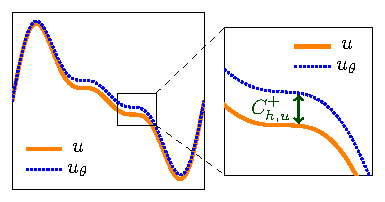
\includegraphics[width=0.6\linewidth]{images/efup/correction_entier/correction.pdf}
    \end{center}
}

\vspace{-8pt}
\only<3>{\begin{center}
    \textcolor{darkred}{\textbf{We hope that the modified problem will give the same results \\
    as the standard one on coarser meshes.}}
\end{center}
}

\end{frame}

\begin{frame}{Convergence analysis}
	\vspace{-10pt}
	\hypersetup{
		citecolor=white,
	}

	\begin{mytheo}{Convergence analysis of the standard FEM \footnotesize\citep{Ern2004TheoryAP}\normalsize}{fem}
		We denote $u_h\in V_h$ the solution of \eqref{eq:weakform} with $V_h$ the standard trial space. Then,
		\vspace{-5pt}
		\begin{equation*}
			| u-u_h|_{H^1} \leqslant C_{H^1} \, h^{k} |u|_{H^{k+1}},
		\end{equation*}
		\begin{equation*}
			\| u-u_h\|_{L^2} \leqslant C_{L^2} \, h^{k+1} |u|_{H^{k+1}}.
		\end{equation*}
	\end{mytheo}
	
	\begin{mytheo}{Convergence analysis of the enriched FEM \footnotesize\citep{ours_2025}\normalsize}{add}
		We denote $u_h^+\in V_h^+$ the solution of \eqref{eq:weakplus} with $V_h^+$ the enriched trial space. Then,
		\vspace{-5pt}
		\begin{equation*}
			| u-u_h^+|_{H^1} \leqslant \fcolorbox{orange}{other!10!white}{$\frac{| u-u_{\theta} |_{H^{k+1}}}{| u |_{H^{k+1}}}$} \left(C_{H^1} \, h^{k} |u|_{H^{k+1}}\right),
		\end{equation*}
		\begin{equation*}
			\| u-u_h^+\|_{L^2} \leqslant \fcolorbox{orange}{other!10!white}{$\frac{| u-u_{\theta} |_{H^{k+1}}}{| u |_{H^{k+1}}}$} \left(C_{L^2} \, h^{k+1} |u|_{H^{k+1}}\right).
		\end{equation*}
	\end{mytheo}

	\hypersetup{
		citecolor=other,
	}

	\footnotesize
	\textcolor{orange}{Gains of the additive approach.}
\end{frame}


\subsection{The heated cavity test case considered}

\begin{frame}{Enriched space using PINN} %\footnote[frame,1]{The $\bm{\mu}$ parameter is fixed in the FE resolution.}}	
    Considering the PINN prior $U_\theta = (\bm{u}_\theta, p_\theta, T_\theta)$, we define the \textcolor{darkred}{mixed finite element space additively enriched} by the PINN as follows:
    
    \begin{center}
        \fcolorbox{darkred}{white}{$M_h^+ = \left\{U_h^+ = U_\theta + C_h^+, \quad C_h^+ \in M_h^{\, 0}\right\}$}
    \end{center}

    with $M_h^{\, 0}=[V_h^{\, 0}]^2 \times Q_h \times W_h^0$,
    $U_h^+ = (\bm{u}_h^+, p_h^+, T_h^+) \in M_h^+$ and $C_h^+ = (\bm{C}_{h,\bm{u}}^+, C_{h,p}^+, C_{h,T}^+)$.

    \vspace{8pt}

    We can then define the three finite element subspaces of $M_h^+$ as follows:
    \begin{minipage}{0.6\linewidth}
        \vspace{-15pt}
        \begin{align*}
            \bm{V}_h^+ &= \left\{\bm{u}_h^+ = \bm{u}_\theta + \bm{C}_{h,\bm{u}}^+, \; \bm{C}_{h,\bm{u}}^+ \in [V_h^{\, 0}]^2\right\}, \\
            Q_h^+ &= \left\{p_h^+ = p_\theta + C_{h,p}^+, \; C_{h,p}^+ \in Q_h\right\}, \\
            W_h^+ &= \left\{T_h^+ = T_\theta + C_{h,T}^+, \; C_{h,T}^+ \in W_h^{\, 0}\right\},
        \end{align*}
        where $\bm{C}_{h,\bm{u}}^+$, $C_{h,p}^+$ and $C_{h,T}^+$ becomes the unknowns.
        
        % \vspace{5pt}
        % \hl{à ajouter : dans quoi vit $U_\theta$ ?}
    \end{minipage}
    \begin{minipage}{0.38\linewidth}
        \centering
        \vspace{5pt}
        \pgfimage[width=0.7\linewidth]{images/efup/correction/correction.pdf}
    \end{minipage}
\end{frame}


\begin{frame}{Weak formulation - Additive approach}
    \textbf{Weak problem :} Find $C_h^+=(\textcolor{Cyan}{\bm{C}_{h,\bm{u}}^+}, \textcolor{blue}{C_{h,p}^+}, \textcolor{ForestGreen}{C_{h,T}^+}) \in M_h^{\, 0}$ s.t., \; $\forall (\bm{v}_h, q_h, w_h) \in M_h^{\, 0}$,

    \vspace{-4pt}
    \footnotesize
    \begin{equation}
        \label{eq:weak_pb_add}
        \hspace{-8pt}\begin{aligned}
            &\int_\Omega \big[(\textcolor{darkred}{\bm{u}_\theta} \cdot \nabla)\textcolor{darkred}{\bm{u}_\theta} + (\textcolor{darkred}{\bm{u}_\theta} \cdot \nabla)\textcolor{Cyan}{\bm{C}_{h,\bm{u}}^+} + (\textcolor{Cyan}{\bm{C}_{h,\bm{u}}^+} \cdot \nabla)\textcolor{darkred}{\bm{u}_\theta} + (\textcolor{Cyan}{\bm{C}_{h,\bm{u}}^+} \cdot \nabla)\textcolor{Cyan}{\bm{C}_{h,\bm{u}}^+} \big] \cdot \bm{v_h} \, d\bm{x} \\
            &\hspace{20pt} +\mu \left(\int_\Omega  \nabla \textcolor{darkred}{\bm{u}_\theta} : \nabla \bm{v}_h \, d\bm{x} + \int_\Omega \nabla \textcolor{Cyan}{\bm{C}_{h,\bm{u}}^+} : \nabla \bm{v}_h \, d\bm{x}\right) + \left(\int_\Omega \nabla \textcolor{darkred}{p_\theta} \cdot \bm{v}_h \, d\bm{x} - \int_\Omega \textcolor{blue}{C_{h,p}^+} \nabla \cdot \bm{v}_h \, d\bm{x}\right)\\
            &\hspace{50pt} - g \int_\Omega (1 + \beta (\textcolor{darkred}{T_\theta} + \textcolor{ForestGreen}{C_{h,T}^+})) \bm{e}_y \cdot \bm{v}_h \, d\bm{x} = 0, \,\text{\footnotesize (momentum)}  \\
            &\int_\Omega q_h \, \big[\nabla \cdot \textcolor{darkred}{\bm{u}_\theta} + \nabla \cdot \textcolor{Cyan}{\bm{C}_{h,\bm{u}}^+}\big] \, d\bm{x} \, + \, 10^{-4} \int_\Omega q_h \, (\textcolor{darkred}{p_\theta} + \textcolor{blue}{C_{h,p}^+}) \, d\bm{x} = 0, \; \text{\footnotesize (incompressibility + penal)} \\
            & \int_\Omega \big[ \textcolor{darkred}{\bm{u}_\theta} \cdot \nabla \textcolor{darkred}{T_\theta} + \textcolor{darkred}{\bm{u}_\theta} \cdot \nabla \textcolor{ForestGreen}{C_{h,T}^+} + \textcolor{Cyan}{\bm{C}_{h,\bm{u}}^+} \cdot \nabla \textcolor{darkred}{T_\theta} + \textcolor{Cyan}{\bm{C}_{h,\bm{u}}^+} \cdot \nabla \textcolor{ForestGreen}{C_{h,T}^+} \big] w_h \, d\bm{x} \\
            & \hspace{40pt} + k_f \left(\int_\Omega \nabla \textcolor{darkred}{T_\theta} \cdot \nabla w_h \; d\bm{x} + \int_\Omega \nabla \textcolor{ForestGreen}{C_{h,T}^+} \cdot \nabla w_h \, d\bm{x} \, w_h \, d\bm{s}\right) = 0, \, \text{\footnotesize (energy)}
        \end{aligned}
        \tag{$\mathcal{P}_h^+$}
    \end{equation}

    \vspace{5pt}
    with \textcolor{darkred}{$U_\theta = (\bm{u}_\theta, p_\theta, T_\theta)$} the PINN prior and some modified boundary conditions.
\end{frame}

\begin{frame}{Newton method - Additive approach}
    \vspace{-5pt}
    We want to solve the non linear system: %\hfill \tiny $N_h$ : number of degrees of freedom.

    \normalsize
    \vspace{-10pt}
    \begin{equation*}
        % \label{eq:nonlinear}
        F_\theta(\vec{C}) = 0 
    \end{equation*}

    \vspace{-2pt}
    with $F_\theta:\mathbb{R}^{N_h} \to \mathbb{R}^{N_h}$ the non linear operator associated to the weak problem \eqref{eq:weak_pb_add} and $\vec{C}\in \mathbb{R}^{N_h}$ the \textcolor{darkred}{correction vector (unknown)}.

	\setcounter{algocf}{1}
    \begin{center}
        \small
        \begin{minipage}{0.9\linewidth}
            \begin{algorithm}[H]
                \SetAlgoLined
                \caption{Newton algorithm \citep{newton_accel_2025}}
                \textbf{Initialization step:} set $\vec{C}^{(0)} = \textcolor{darkred}{0}$\;
                \For{\( n \ge 0 \)}{
                    Solve the linear system \( F_\theta(\vec{C}^{(n)}) + F_\theta'(\vec{C}^{(n)}) \delta^{(n+1)} = 0 \) for \( \delta^{(n+1)} \)\;
                    Update \( \vec{C}^{(n+1)} = \vec{C}^{(n)} + \delta^{(n+1)} \)\;
                }
            \end{algorithm}
        \end{minipage}
    \end{center}
    
    \vspace{3pt}
    \textbf{Advantage compared to PINN initialization\footnote[frame,1]{Taking $U_\theta$ and $C_h^+$ in the same space, additive approach is exactly the same as the PINN initialization.}:} %\refappendix{frame:comp}

    \vspace{-2pt}
    \begin{center}
        \textcolor{darkred}{$u_\theta$ is not required to live in the same discrete space as $C_h^+$}.
    \end{center}
    \vspace{8pt}
\end{frame}